\documentclass[12pt,titlepage]{article}

\usepackage[top=1.75in,left=1.5in,right=1.5in,bottom=1.25in,verbose]{geometry}%footskip=.25in,
\usepackage{graphicx}
\usepackage{rotating}
\usepackage{amssymb,amsmath}\allowdisplaybreaks[4]
\usepackage{multirow}
\usepackage{fancyhdr}
\usepackage{overpic}
\usepackage{epsfig}
\usepackage{setspace}
\usepackage{makeidx}
\usepackage{epsfig}
\usepackage{paralist}
\usepackage{appendix}
\usepackage{changebar}
\usepackage[round]{natbib}

\newcounter{funnum}
\newcommand{\fthefunnum}{F\thefunnum}
\newcommand{\fref}[1]{F\ref{#1}}

\newcounter{nfnum}
\newcommand{\nthenfnum}{N\thenfnum}
\newcommand{\nref}[1]{N\ref{#1}}

\newcounter{goalnum}
\newcommand{\gthegoalnum}{G\thegoalnum}
\newcommand{\gref}[1]{G\ref{#1}}

\newcounter{assnum}
\newcommand{\atheassnum}{A\theassnum}
\newcommand{\aref}[1]{A\ref{#1}}

\newcounter{tmnum}
\newcommand{\tmthetmnum}{TM\thetmnum}
\newcommand{\tmref}[1]{TM\ref{#1}}

\newcounter{ddnum}
\newcommand{\dtheddnum}{D\theddnum}
\newcommand{\dref}[1]{D\ref{#1}}

\newcounter{acnum}
\newcommand{\actheacnum}{AC\theacnum}
\newcommand{\acref}[1]{AC\ref{#1}}

\newcounter{ucnum}
\newcommand{\uctheucnum}{UC\theucnum}
\newcommand{\uref}[1]{UC\ref{#1}}

\newcounter{mnum}
\newcommand{\mthemnum}{M\themnum}
\newcommand{\mref}[1]{M\ref{#1}}

\newcounter{qfnum}
\newcommand{\qftheqfnum}{QF\theqfnum}
\newcommand{\qfref}[1]{QF\ref{#1}}

\newcounter{casenum}
\newcommand{\cthecasenum}{TC\thecasenum}
\newcommand{\cref}[1]{TC\ref{#1}}

\newcommand{\mi}[1]{#1\index{#1}}
%\makeindex

\addtocounter{secnumdepth}{3}

\newcommand{\colAwidth}{0.36\textwidth}
\newcommand{\colBwidth}{0.45\textwidth}
\newcommand{\firstCol}{0.17\textwidth}
\newcommand{\secondCol}{0.7\textwidth}
\newcommand{\colOne}{0.1\textwidth}
\newcommand{\colTwo}{0.15\textwidth}

\DeclareGraphicsRule{.jpg}{eps}{}{}

\pagestyle{fancy}
\renewcommand{\headrulewidth}{0pt}
\renewcommand{\footrulewidth}{0pt}
\fancyhf{} \fancyfoot[C]{\thepage} \fancyhead[C]{\itshape Wen Yu -- McMaster University -- Computing and Software}

\setlength{\parindent}{0.5in}

\newcommand{\HRule}{\rule{\linewidth}{0.5mm}}
%\doublespacing

\author{Wen Yu}

\begin{document}

\begin{titlepage}

% Fonts for the title page
\newcommand{\texttl}{\textsf} %font for the title (Emil's version is \textsf)
\newcommand{\textau}{\textsf} %font for the authors, date, etc. (Emils version is \textsc)

\begin{center}
 
\HRule \\[0.4cm]
{ \huge \bfseries \texttl{Software Requirements Specification for a Parallel Mesh Generation Toolbox}}\\[0.4cm]
 
\HRule \\[2cm]

\textau{\LARGE Wen Yu}\\[2cm]
 
\textau{\LARGE {September 2008}}
 
\vfill
 
% Bottom of the page
%\includegraphics[width=0.27\textwidth]{logo.pdf}
\hfill
\textau{\LARGE
\raisebox{2pt}{\begin{tabular}[b]{r}
\raisebox{8pt}{Computing and Software} \\
McMaster University \end{tabular}}
}
\end{center}

\end{titlepage}

\tableofcontents

\newpage

\section{Reference Material}
\subsection{Table of Symbols, Abbreviations and Acronyms}

\subsubsection{Symbols}
\begin{tabular}{p{\firstCol}p{\secondCol}} 
$\Omega$ & a closed bounded domain in $\mathbb{R}^{2}$  \\
$\Omega^{*}$ & a mesh covering the domain bounded by $\Omega$\\
$K$ & a simple shape, such as a line segment in 1D, a triangle or a quadrilateral in 2D, or a tetrahedron or hexahedron
in 3D\\
$M^{\mbox{IN}}$ & an input mesh\\
$M^{\mbox{OUT}}$ & an output mesh\\
$I$ & instructions on how a mesh should be \\
 & refined/coarsened
\end{tabular}
%\newpage

\subsubsection{Abbreviations and Acronyms}
\begin{tabular}{p{\firstCol}p{\secondCol}} 
1D & One Dimensional Space\\
2D & Two Dimensional Space\\
3D & Three Dimensional Space\\
FEA & Finite Element Analysis\\
HPC & High Performance Computing\\
PDE & Partial Differential Equation\\
PMGT & Parallel Mesh Generation Toolbox\\
SHARCNET & Shared Hierarchical Academic Research Computing Network\\
SRS & Software Requirements Specification\\
AOMD & Algorithm Oriented Mesh Database\\
\end{tabular}
\newpage

\subsection{Index of Requirements}
CoarseningMesh, \pageref{CoarseningMesh}\\
Conformal, \pageref{Conformal}\\\\
DomainDimension, \pageref{DomainDimension}\\\\
ElmShape, \pageref{ElmShape}\\
ElmTopology, \pageref{ElmTopology}\\
ElmUniqueID, \pageref{ElmUniqueID}\\
Exception, \pageref{Exception}\\\\
Help, \pageref{Help}\\\\
InputDefinition, \pageref{InputDefinition}\\\\
LookAndFeel, \pageref{LookAndFeel}\\\\
Maintainability, \pageref{Maintainability}\\
MeshType, \pageref{MeshType}\\\\
OutElmOrder, \pageref{OutElmOrder}\\
OutputStorage, \pageref{OutputStorage}\\
OutVertexOrder, \pageref{OutVertexOrder}\\\\
Performance, \pageref{Performance}\\
Portability, \pageref{Portability}\\
Precision, \pageref{Precision}\\\\
RCInstruction, \pageref{RCInstruction}\\
RefiningMesh, \pageref{RefiningMesh}\\
RefiningOrCoarsening, \pageref{RefiningOrCoarsening}\\\\
Usability, \pageref{Usability}\\\\
VertexUniqueID, \pageref{VertexUniqueID}
%\printindex
\newpage

\section{Introduction \label{AreqSecIntro}}

This section gives an overview of the Software Requirements Specification (SRS) for a Parallel Mesh Generation Toolbox (PMGT). First, the purpose of the document is provided. Second, the scope of PMGT is identified. Third, some terminology for software engineering and mesh generation are defined. Finally, the organization of the document is summarized. The Table of Symbols, Abbreviation and Acronyms, and Index of Requirement are given at the beginning of the SRS.

\subsection{Purpose of the Document}
This SRS provides a black-box description of PMGT. The intended audience of the SRS is the development team and the users of PMGT.

\subsection{Scope of the Software Product}
PMGT provides a library that will be embedded into a larger application, such as a finite element analysis (FEA) program. 
\begin{itemize}
\item The input of PMGT is an existing mesh $M^{\mbox{IN}}$ with instructions $I$ provided by the user on how the mesh should be refined/coarsened.
\item PMGT refines/coarsens $M^{\mbox{IN}}$ according to the supplied instructions $I$ on how the mesh should be refined/coarsened.
\item PMGT will take advantage of parallel computation.
\item The output of PMGT is a refined/coarsened mesh $M^{\mbox{OUT}}$.
\end{itemize}
Note that depending on the given instruction, PMGT can either refine or coarsen the given mesh, but cannot do both at the same time. That is, any individual transition from $M^{\mbox{IN}}$ to $M^{\mbox{OUT}}$ will only do one of refining or coarsening. The embedding application will have access to reading the mesh information, such as information on the position of vertices and on the vertices that define a given element. However, the application cannot directly change any mesh data, except for the information indicating which elements should be refined/coarsened. 

\subsection{Terminology Definition}
This subsection provides the definitions for terminology used in the SRS. There are two classes of terminology. One relates to software engineering, and the other relates to mesh generation. The definitions are listed in alphabetical order.
\subsubsection{Software Engineering Related Terminology\label{AreqSEterm}}
\begin{description}

\item[Constraint:] A statement that expresses measurable bounds for an element or function of the system. That is, a constraint is a factor that is imposed on the solution by force or compulsion and may limit or modify the design changes. \citep{IEEE1998}

\item[Context:] The boundaries between the system that we intend to build and the people, organizations, other system and pieces of technology that have a direct interface with the system. \citep{Volere2001}

\item[Functional Requirements:] Functional requirements define precisely what input are expected by the software, what outputs will be generated by the software, and the details of relationships that exist between those inputs and outputs. In short, functional requirements describe all aspects of interface between the software and its environment (that is, hardware, humans, and other software). \citep{Davis1990}

\item[Goal:] Goals capture, at different levels of abstraction, the various objectives the system under
consideration should achieve. \citep{Lamsweerde2001}

\item[Non-functional Requirements:] Non-functional requirements define the overall qualities or attributes to be exhibited by the resulting software system. \citep{Davis1990}

\item[Requirements:] A software requirement is: \begin {inparaenum}[\itshape i\upshape)]
\item a condition or capability needed by a user to solve a problem or achieve an objective;
\item a condition or capability that must be met or possessed by a system or system component to satisfy a contract,
standard, specification, or other formally imposed document; or, 
\item a documented representation of a condition or capability as in the above two definitions.
\end{inparaenum} \citep{IEEE2000}

\item[Software Engineering:] Software Engineering is the application of a systematic, disciplined, quantifiable approach to the development, operation, and maintenance of software. \citep{IEEE1990}

\item[Software Requirements Specification:] A Software Requirements Specification (SRS) is a document containing a complete description of what the software will do without describing how it will do it. \citep{Davis1990}

\item[System:] An interdependent group of people, objects, and procedures constituted to achieve defined objectives or some operational role by performing specified functions. \citep{IEEE1998}

\item[System Context:] System Context documents the relationships between the system being specified and other human and computer systems. \citep{Sommerville1992}

\item[User:]The person, or persons, who operate or interact directly with the product. \citep{IEEE2000}

\end{description}

\subsubsection{Mesh Generation Related Terminology\label{AreqMGterm}}
\begin{description}

%\item [Aspect Ratio:] The aspect ratio of a simplex is defined as its maximum side length divided by its minimum altitude. \citep{Mitchell2000}
%The aspect ratio of a convex body is the ratio between its longest dimension and its shortest dimension.

\item [Cell:] Another name for an element, as defined in page \pageref{AreqElmDef}.

\item[Conformal Mesh:] A conformal mesh is a mesh (defined on page \pageref{def_mesh}) following the definition of a mesh, with the addition of the
following property:\\
The intersection of two elements in the mesh $\Omega^{*}$ is either the empty set, a vertex, an edge or a face (when the
dimension is 3). \citep{FreyAndGeorge2000}

\item [Connectivity:] There are two types of connectivity, one for the mesh and one for a mesh element:
\begin{enumerate}
\item ``The connectivity of a mesh is the definition of the connection between its vertices.''~\citep{FreyAndGeorge2000}
\item ``The connectivity of a mesh element is the definition of the connections between the vertices at the element
level.''~\citep{FreyAndGeorge2000}
\end{enumerate}

\item [Domain:] The area or volume that is to be discretized.  The domain is sometimes referred to as the
computational domain. \citep{Smith2004}


\item [Edge:] An edge is a line segment between two vertices.

\item [Element \label{AreqElmDef}:] The original domain is discretized into smaller, usually simpler, shapes called elements. 
The typical shapes for elements in 1D is a line, in 2D is a triangle or a quadrilateral, and in 3D a tetrahedron or a
hexahedron.  Elements are also called cells. \citep{Smith2004}

\item [Embedding Application:] The software that uses PMGT.

\item [Face:] A face is a maximal connected subset of the plane without vertices inside the subset. In 2D, a face is a cell.\citep{FreyAndGeorge2000}

\item [Hybrid Mesh:] A mesh is said to be hybrid if it includes some elements with a different spatial dimension. \citep{FreyAndGeorge2000}

\item[Mesh:] \label{def_mesh}
In \citet{Smith2004}, a mesh is defined as follows:\\
Let $\Omega$ be a closed bounded domain in $\mathbb{R}$ or $\mathbb{R}^2$ or $\mathbb{R}^3$
and let $K$ be an element.  A mesh of $\Omega$, denoted by $\Omega^{*}$, has the following properties:
\begin{enumerate}
\item $\Omega \approx \cup(K | K \in \Omega^{*} : K)$, where $\cup$ is first closed and then opened
\item the length of every element $K$, of dimension 1, in $\Omega^{*}$ is greater than zero
\item the interior of every element $K$, of dimension 2 or greater, in $\Omega^{*}$ is nonempty
\item the intersection of the interior of two elements is empty
\end{enumerate}
The only difference between above definition and the definition given by \citet{FreyAndGeorge2000} is that equality (=) had been changed to approximate equality ($\approx$).

\item [Mesh Generation:] The automatic mesh generation problem is that of attempting to define a set of elements to best describe a geometric domain, subject to various element size and shape criteria. \citep{Smith2004}

\item [Mixed Mesh:] A mesh is said to be mixed if it includes some elements of a different geometric nature. \citep{FreyAndGeorge2000}

\item [Structured Mesh:] The mesh in which the local organization of the grid points and the form of the grid cells do not depend on their position but are defined by a general rule.  There is a pattern to the topology that repeats. 
\citet{FreyAndGeorge2000} say, ``a mesh is called structured if its connectivity is of the finite difference type.'' 
They go on to remark, ``Peculiar meshes other than quad or hex meshes could have a structured connectivity.  For
instance, one can consider a classical grid of quads where each of them are subdivided into two triangles using the same
subdivision pattern.''

\item [Topology:] ``The topology of a mesh element is the definition of this element in terms of its faces and edges,
these last two being defined in terms of the element's vertices.''~\citep{FreyAndGeorge2000}\\
The topology of a mesh is the set of topologies of its constitute mesh elements.

\item [Unstructured Mesh:] The mesh whose element connectivity of the neighbouring grid vertices varies from point to
point.  Any mesh that is not structured is an unstructured mesh. \citep{Smith2004}

\item [Vertices:] The locations that define the shape of the cells.  In 1D the vertices are the end-points of the
elements.  For 2D and 3D elements the vertices correspond to the location in space that defines the intersection of
the edges of an element. \citep{Smith2004}

\end{description}


\subsection{Organization of the Document}
This SRS follows the template introduced by~\cite{Lai2004}. Lai's template targets an SRS for scientific computing software. In particular, the example shown is for engineering mechanics software, such as software to analyze beams. In the current work, Lai's template is modified to fit PMGT, which is a more general purpose software. For example, the instanced model section of Lai's template is removed since PMGT is not designed for solving a specific physical problem.
 
Section \ref{AreqSecIntro} (this section) is an introduction to the SRS. 
The rest of the document is arranged as follows. Section \ref{AreqSecGSD} provides the general information about the system. Section \ref{AreqSecSSR} is the major part of the SRS. All functional requirements and non-functional requirements of the software are presented in this section. Section \ref{AreqSecOSI} discusses some other system issues. Section \ref{AreqSecTM} gives a traceability matrix that summaries the association of each requirement with goals, assumptions, theoretical models and data definitions introduced in \ref{AreqSecSSR}. This SRS also contains the list of possible changes in the requirements and values of auxiliary constants. The references are listed at the end of this document.  

\section{General System Description \label{AreqSecGSD}}

This section describes the general information about the system. The interfaces between the system and its environment are defined first. Then the characteristics of potential users are discussed. At end of this section, some system constraints are described.

\subsection{System Context}
The software to be built is a library tool that will be called by other applications. There is no direct interaction between the system and the end users. Users of the embedding application, such as an FEA program, provide some parameters directly to the FEA program. Some of these parameters are passed to PMGT by the FEA program. The interface between PMGT and the embedding application should only show what PMGT can do and hide the information about how to do it. Therefore, users who are not experts in mesh generation or in parallel processing will be able to use this toolbox.  %The characteristics of users of PMGT will be described in the Section \ref{userchar}.
\begin{figure}[ht]
\centering
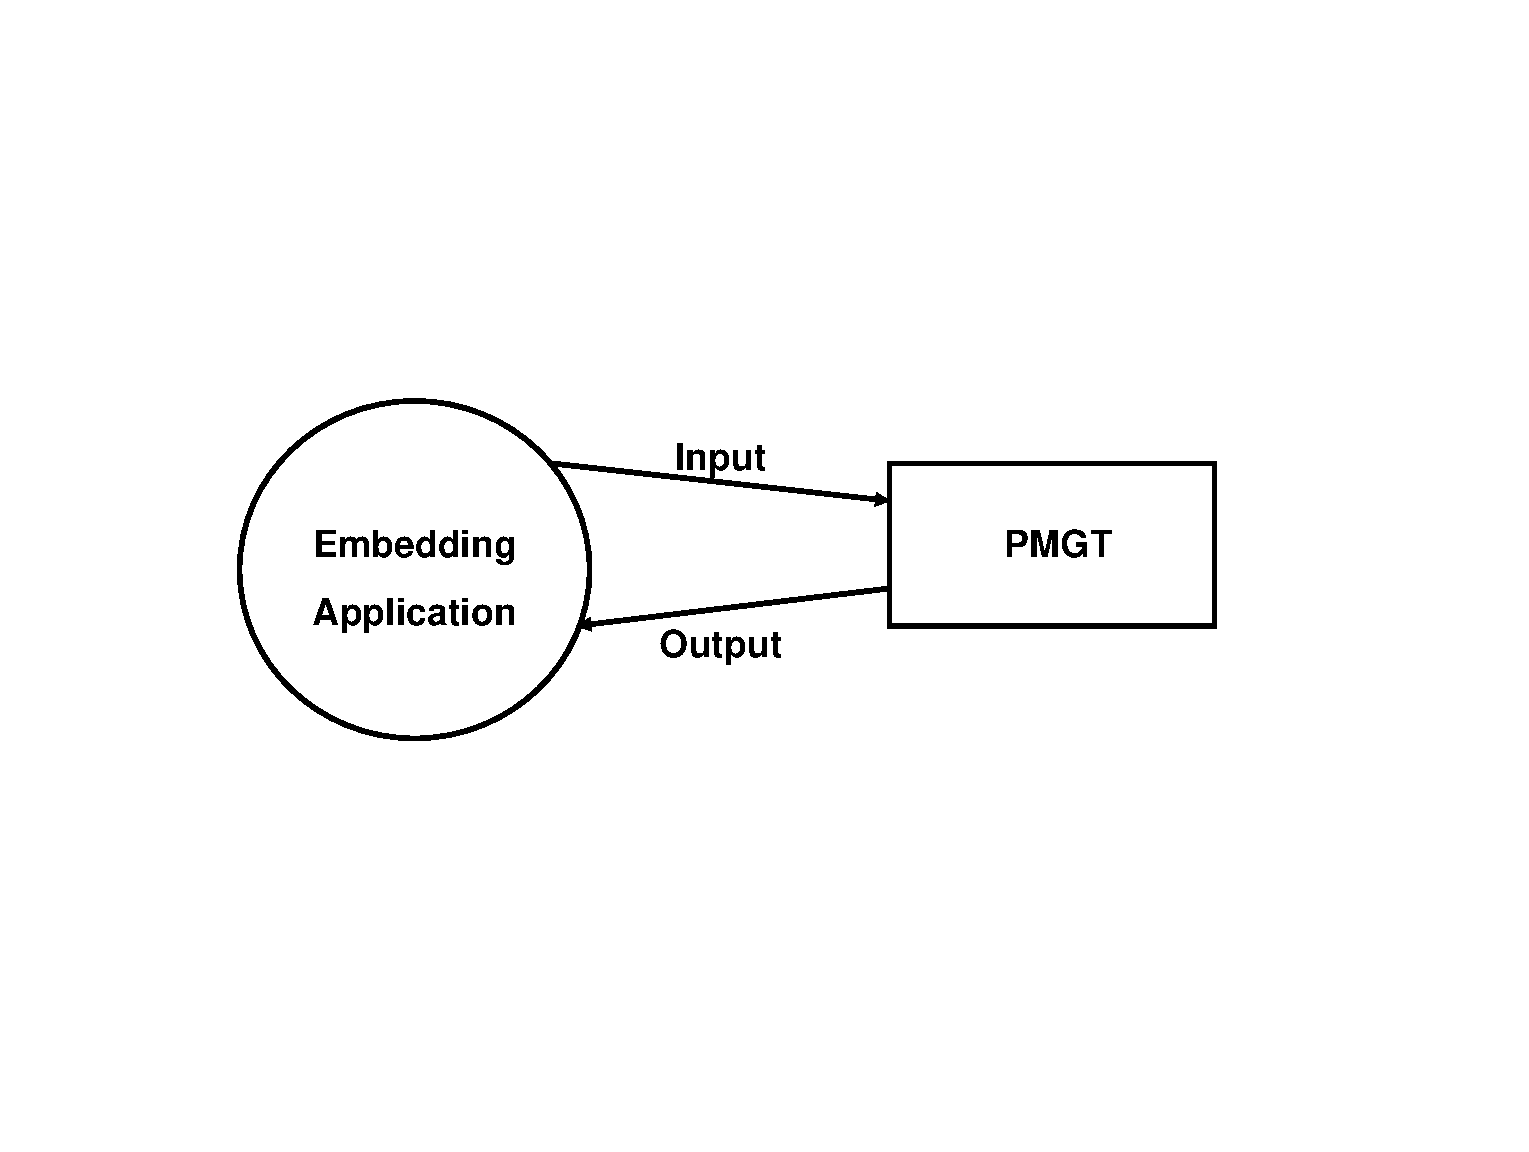
\epsfig{file=syscon.eps, width=\textwidth}
\caption{System Context Diagram}
\label{AreqSyscon}
\end{figure}

Figure~\ref{AreqSyscon} shows the context that PMGT will normally fit into.
A circle represents an external entity outside the system, an embedding application in this case. The rectangle is the system itself. Arrows represent the data flows between them.

The \emph{input}: $M^{\mbox{IN}}\times I$ 

The \emph{output}: $M^{\mbox{OUT}}$.

PMGT has the following function:
\begin{quote}
A mesh $M^{\mbox{IN}}$ and some refining/coarsening instructions $I$ are given. PMGT generates a refined/coarsened mesh $M^{\mbox{OUT}}$ according to the instructions $I$. 
\end{quote}
%\begin{quotation}

%\end{quotation}

\subsection {User Characteristics}\label{AreqUserchar}
The target user group of PMGT includes both software designers, who intend to embed this library in their applications, and theoreticians, who are involved in parallel mesh generation. A user of PMGT is expected to be familiar with the notion/knowledge of mesh creation. PMGT is a library used by other applications. Therefore, users should not be novices in terms of software design. The prerequisite software design knowledge are equivalent to that of a senior undergraduate student in science or engineering who took an introductory course on programming. For example, they should be comfortable with compilation of the programming language in which PMGT is written, be familiar with embedding a library in their software, $etc.$

\subsection{System Constraints}
This system is intended to be built on the Shared Hierarchical Academic Research Computing Network (SHARCNET). 
SHARCNET is structured as a ``cluster of clusters'' across South Central Ontario, designed to meet the computational needs of researchers in a diverse number of research areas and to facilitate the development of leading-edge tools for high performance computing (HPC) grids.

Large production clusters, located at the Universities of Western Ontario, Guelph and McMaster, house over 400 HP/Compaq
Alpha processors and large symmetric multiprocessor computers. Windsor and Wilfrid Laurier host smaller development
clusters (8 processors), which enable researchers to develop and test code before moving to one of the larger clusters.
A glance of SHARCNET systems is shown in Table \ref{AreqSharcnet}. Note that the network is constantly being updated. Detailed information can be found at \citet{sharcnet2006}.
\begin{table}[htbp]
\centering
\begin{tabular}{p{0.2\textwidth}|p{0.2\textwidth}|p{0.1\textwidth}|p{0.1\textwidth}|p{0.25\textwidth}} 
\hline \hline
System & Make & Type & CPUs & OS \\
\hline
bala & Compaq & Cluster & 8 & Red Hat Linux 7.2\\
cat & Unknown & Cluster & 162 & Red Hat Linux 8 \\
goblin & Sun & Cluster & 56 & Fedora Core 2 \\
hammerhead & Compaq & Cluster & 112 & Red Hat Linux 7.2 \\
idra & Compaq SC & Cluster & 128 & Tru64 \\
mako & HP & Cluster & 16 & Fedora Core 2 \\
tiger & Compaq & Cluster & 8 & Red Hat Linux 7.2 \\
typhon & Compaq & SMP & 16 & Tru64 \\
wobbe & Unknown & Cluster & 193 & Red Hat Linux 8 \\
TOTALS & & & 699 \\
\hline \hline
\end{tabular} 
\caption{A Glance at the SHARCNET System}
\label{AreqSharcnet}
\end{table}

\section{Specific System Requirements \label{AreqSecSSR}} 

This section describes the system requirements in detail. After the problem is clearly and unambiguously stated, some solution characteristics are specified. Non-functional requirements are also included in this section. The symbol $:=$ is used to indicate type definition. The notation for set building and expressions used in this section follows \citet{Gries1993}. To define the notation, first let $x$ be a list of dummies, $t$ a type, $R$ a predicate, $E$ an expression, $*$ an operator, and $P$ a predicate. Notation $\{ x:t\ |\ R:E\}$ represents a set of values that result from evaluating $E[x:=v]$ in the state for each value $v$ in $t$ such that $R[x:=v]$ holds in that state. Expression $(*x:t\ |\ R:P)$ denotes the application of operator $*$ to the values $P$ for all $x$ in $t$ for which range $R$ is true. 

\subsection{Problem Description \label{AreqSecPD}}
The problems (goals) specified in this subsection represent ideal general models. The problems are simplified by introducing some assumptions, which are listed in Section \ref{AreqSolution}.

\subsubsection{Background Overview}
Many physical problems of importance to scientists and engineers are modeled as a set of Partial Differential Equations (PDEs). In most practical cases, it is necessary to solve the PDEs numerally. Numerical methods to solve PDEs frequently require that the domain of interest be divided into a mesh, which is a set of small, simple elements that cover the computational domain. In some applications, a single mesh is generated and used  many times; in this case the processing time spent on mesh construction is not critical and a relatively slow, sequential algorithm suffices \citep{Ruppert1993}. However, some applications need adaptive meshing, which requires that the meshes be generated once and then modified many times. For instance, adaptive meshing is used for reliable Finite Element Analysis (FEA) using a posterrori error estimation \citep{Zienkiewicz2005}. The increased mesh interaction for adaptive meshing means an increased need for speed of managing the mesh data which suggest employing parallel processing techniques. Although generating a mesh using multiple processors is complicated, it can offer considerable speed-up over sequential processing. In addition, some FEA applications are implemented on multiple processors. If the adaptive mesh can be generated in multiple processors as well, the mesh data can remain on the local processors. Potentially, time to be used will be significantly reduced. 

\subsubsection{Goal Statements}
There are two related goals for PMGT.
\begin{description}
\item[\refstepcounter{goalnum}\gthegoalnum \label{gRefining}:] Given a mesh $M^{\mbox{IN}}$ and instructions $I$ on how to refine the mesh, PMGT should generate a refined mesh $M^{\mbox{OUT}}$ according to the instructions $I$.
\item[\refstepcounter{goalnum}\gthegoalnum \label{gCoarsening}:]Given a mesh $M^{\mbox{IN}}$ and instructions $I$ on how to coarsen the mesh, PMGT should generate a coarsened mesh $M^{\mbox{OUT}}$ according to the instructions $I$.
\end{description}

\subsection{Solution Characteristics Specification\label{AreqSolution}}
The goals stated in the last section are too general to achieve. In this section, the assumptions are specified first to reduce the scope of the software. Second, the theoretical models for the goals are described. Third, data definitions are given to assist with defining the theoretical models. Finally, the system behaviour is summarized.     
\subsubsection{Assumptions}
\begin{description}
\item [\refstepcounter{assnum} \atheassnum \label{aDimension}:]PMGT focuses on a 2D domain.
\item[\refstepcounter{assnum} \atheassnum \label{aClosed}:]The input and output meshes are bounded.
\item [\refstepcounter{assnum} \atheassnum \label{aUnstructured}:]The input and output meshes are unstructured.
\item[\refstepcounter{assnum} \atheassnum \label{aConformal}:]The input and output meshes are conformal.
\item[\refstepcounter{assnum} \atheassnum \label{aElmShape}:]The elements of input and output meshes are triangles.
\item[\refstepcounter{assnum} \atheassnum \label{aValidMesh}:] The initial mesh is valid.
\end{description}

\subsubsection{Theoretical Model}
The theoretical models corresponding to the goals given in Section \ref{AreqSecPD} describes the relationship between the input mesh ($M^{\mbox{IN}}$) and the output mesh ($M^{\mbox{OUT}}$). The meshes are assumed to be embedded in a 2D space. 
\begin{description}
\item[\refstepcounter{tmnum} \tmthetmnum \label{tmRefining}:] Refining Mesh
\begin{description}
\item [\emph{Input}:] $M^{\mbox{IN}}$: {\tt MeshT}, $I$: {\tt RCinstructionT}
\item [\emph{Output}:] $M^{\mbox{OUT}}$: {\tt MeshT}
\end{description}
The following behavior is specified: 
\begin{itemize}
\item {\it Refined}($M^{\mbox{OUT}},\ M^{\mbox{IN}}$)
\end{itemize}
That is, the output mesh is a refined version of the input mesh.
\item[\refstepcounter{tmnum} \tmthetmnum \label{tmCoarsening}:] Coarsening Mesh
\begin{description}
\item [\emph{Input}:] $M^{\mbox{IN}}$: {\tt MeshT}, $I$: {\tt RCinstructionT}
\item [\emph{Output}:] $M^{\mbox{OUT}}$: {\tt MeshT}
\end{description}
The following behavior is specified: 
\begin{itemize}
\item {\it Coarsened}($M^{\mbox{OUT}},\ M^{\mbox{IN}}$)
\end{itemize}
That is, the output mesh is a coarsened version of the input mesh.
\end{description}

\subsubsection{Data Definitions}
The data definitions below are organized so that a definition listed in the beginning may be used to define a data item  listed after it.
\begin{description} 
\item [VertexT (\refstepcounter{ddnum} \dtheddnum \label{dVertexT}):] A vertex is represented by two real numbers, which are its $x$ coordinate and $y$ coordinate. More formally,\\
{\tt VertexT} := tuple of ($x: \mathbb{R},\  y: \mathbb{R}$).

\item [EdgeT (\refstepcounter{ddnum} \dtheddnum \label{dEdgeT}):] An edge is represented by a set of {\tt VertexT}. More formally,\\
{\tt EdgeT} := set of {\tt VertexT}.

\item [ValidEdge (\refstepcounter{ddnum} \dtheddnum \label{dValidEdge}):] An edge is valid if the edge is a line segment (that is, the set has two elements). More formally, \\
{\it ValidEdge}: {\tt EdgeT} $\rightarrow \mathbb{B}$\\
{\it ValidEdge}($e$: {\tt EdgeT}) $\equiv \# e = 2$

\item [CellT (\refstepcounter{ddnum} \dtheddnum \label{dCellT}):] A cell is represented by a set of $VertexT$. More formally, \\
{\tt CellT} := set of {\tt VertexT}

\item [Area (\refstepcounter{ddnum} \dtheddnum \label{dArea}):] The area of a triangle whose apexes are elements of a cell. More formally, \\
{\it Area}: {\tt CellT} $\rightarrow \mathbb{R}$\\
{\it Area}($c$: {\tt CellT}) $\equiv \Sigma v1,v2,v3$: {\tt VertexT} $|\ v1\in c \wedge v2\in c \wedge v3\in c \\
\wedge v1\neq v2 \wedge v2\neq v3 \wedge v3\neq v1:\\
\frac{1}{12}* |v1.x*v2.y - v2.x*v1.y +\\
v2.x*v3.y - v3.x*v2.y +\\
v1.x*v3.y - v3.x*v1.y |$

\item [ValidCell (\refstepcounter{ddnum} \dtheddnum \label{dValidCell}):] A cell is valid if the cell is a triangle (that is , the set has three elements) and the area of the triangle is greater than zero. More formally, \\
{\it ValidCell}: {\tt CellT} $\rightarrow \mathbb{B}$\\
{\it ValidCell}($c$: {\tt CellT}) $\equiv \# c = 3 \wedge$ {\it Area}($c$) $\geq 0$

\item [MeshT (\refstepcounter{ddnum} \dtheddnum \label{dMeshT}):] A mesh is represented by a set of cells. More formally,\\
{\tt MeshT} := set of {\tt CellT}.

\item [OnEdge (\refstepcounter{ddnum} \dtheddnum \label{dOnEdge}):] Checks if a vertex is on the line segment between  two vertices (exclusive) of an edge. More formally,\\
{\it OnEdge}: {\tt VertexT} $\times$ {\tt EdgeT} $\rightarrow \mathbb{B}$\\
{\it OnEdge}($v$: {\tt VertexT}, $e$: {\tt EdgeT}) $\equiv \exists\ v1,\ v2$: {\tt VertexT} $|\\
 v1 \in e \wedge v2 \in e \wedge v1 \neq v2 \wedge v \neq v1 \wedge v \neq v2:\\
(v1.x < v.x \leq v2.x \wedge \\(v.y-v1.y)/(v.x-v1.x)=(v2.y-v1.y)/(v2.x-v1.x))$

\item [BelongToCell (\refstepcounter{ddnum} \dtheddnum \label{dBelongToCell}):] Checks if an edge belongs to a cell. More formally, \\
{\it BelongToCell}: {\tt VertexT} $\times$ {\tt CellT} $\rightarrow \mathbb{B}$\\
{\it BelongeToCell}($e$: {\tt EdgeT}, $c$: {\tt CellT}) $\equiv \forall\ v$: {\tt VertexT} $|\ v\in e: v\in c$

\item [Inside (\refstepcounter{ddnum} \dtheddnum \label{dInside}):] Checks if a point (of type VertexT) is inside of a cell. The {\em inside} checking is false if the point is on an edge of the cell or the point is a vertex of the cell. (The algorithm to check if a point is inside a polygon is from \citet{Blackpawn}.) More formally,\\
{\it Inside}: {\tt VertexT} $\times$ {\tt CellT} $\rightarrow \mathbb{B}$\\
{\it Inside}($v$: {\tt VertexT}, $c$: {\tt CellT}) $\equiv \exists\ v1,\ v2,\ v3$: {\tt VertexT} $|\\
v1\in c \wedge v2\in c \wedge v3\in c \wedge v1\neq v2 \wedge v2\neq v3 \wedge v3 \neq v1:\\
((v.y-v1.y)*(v2.x-v1.x)-(v.x-v1.x)*(v2.y-v1.y))*\\
((v.y-v2.y)*(v3.x-v2.x)-(v.x-v2.x)*(v3.y-v2.y)) > 0 \wedge \\
((v.y-v2.y)*(v3.x-v2.x)-(v.x-v2.x)*(v3.y-v2.y))*\\
((v.y-v3.y)*(v1.x-v3.x)-(v.x-v3.x)*(v1.y-v3.y)) > 0$

\item [Vertices (\refstepcounter{ddnum} \dtheddnum \label{dVertices}):] A set of all vetices of the mesh. More formally,\\
{\it Vertices}: {\tt MeshT} $\rightarrow$ set of {\tt VertexT}\\
{\it Vertices}($m$: {\tt MeshT}) $\equiv$ \{$v$: {\tt VertexT} $|$ ($\forall\ c$: {\tt CellT} $|\ c\ \in m :v\ \in c):v\}$

\item [Edges (\refstepcounter{ddnum} \dtheddnum \label{dEdges}):] A set of all edges of the mesh. More formally, \\
{\it Edges}: {\tt MeshT} $\rightarrow $ set of $EdgeT$\\
{\it Edges}($m$: {\tt MeshT}) $\equiv \{v1,\ v2$: {\tt VertexT} $|\ (\forall c$: {\tt CellT} $|\ c \in m:\\ v1 \in c \wedge v2 \in c \wedge v1 \neq v2):\{v1, v2\}\}$
 
\item [BoundaryEdges (\refstepcounter{ddnum} \dtheddnum \label{dBoundaryEdges}):]A set of edges are boundary edges if they form a boundary of a mesh. More formally,\\
{\it BoundaryEdges}: {\tt MeshT} $\rightarrow $ set of $EdgeT$\\
{\it BoundaryEdges}($m$: {\tt MeshT}) $\equiv \{ b$: {\tt EdgeT} $|\ b\in$ {\it Edges}($m$) $\wedge \\
(\# \{c$: {\tt CellT} $|\ c\in m \wedge$ {\it BelongToCell}({\it b, c}): $c\}=1$): $b\}$

\item [BoundaryVertices (\refstepcounter{ddnum} \dtheddnum \label{dBoundaryVertices}):] A set of boundary vertices of the mesh. More formally,\\
{\it BoundaryVertices}: {\tt MeshT} $\rightarrow$ set of {\tt VertexT}\\
{\it BoundaryVertices}($m$: {\tt MeshT}) $\equiv \\
\{v$: {\tt VertexT} $|\ v \in$ {\it BoundaryEdges}($m$): $v\}$

\item [Bounded (\refstepcounter{ddnum} \dtheddnum \label{dBounded}):] A mesh is bounded if the boundary edges form a closed polygon(all vertices of boundary edges belong to exactly two boundary edges). More formally, \\
{\it Bounded}: {\tt MeshT} $\rightarrow \mathbb{B}$\\
{\it Bounded}($m$: {\tt MeshT}) $\equiv \forall v$: {\tt VertexT} $|\ v\in$ {\it BoundaryVertices}($m$): \\
($\# \{e$: {\tt EdgeT} $|\ e \in$ {\it BoundaryEdge}($m$) $\wedge v\in e: e\}=2)$

\item [Conformal (\refstepcounter{ddnum} \dtheddnum \label{dConformal}):] In 2D, a mesh is conformal if the intersection of any two cells is either a vertex or an edge or empty. More formally,\\
{\it Conformal}: {\tt MeshT} $\rightarrow \mathbb{B}$\\
{\it Conformal}($m$: {\tt MeshT}) $\equiv \forall c1, c2$: {\tt CellT} $|\ c1\in m \wedge c2\in m \wedge c1\neq c2 : \\
(\exists e$: {\tt EdgeT} $|\ e\in$ {\it Eeges}($m$): $(\exists v:$ {\tt VertexT} $|\ v\in$ {\it Vertices}($m$):\\
$(c1\cap c2 = e \vee c1\cap c2 = v \vee c1\cap c2 = \emptyset) \wedge (\neg$ {\it OnEdge(v, e))  ))}

\item [NoInteriorIntersect (\refstepcounter{ddnum} \dtheddnum \label{dNoInteriorIntersect}):] NoInteriorIntersect is true if a point in space (of type VertexT) is inside only one cell of the mesh. More formally,\\
{\it NoInteriorIntersect}: {\tt MeshT} $\rightarrow \mathbb{B}$\\
{\it NoInteriorIntersect}($m$: {\tt MeshT}) $\equiv \forall c1, c2$: {\tt CellT} $|\\ c1\in m \wedge c2\in m \wedge c1 \neq c2:
 (\forall v$: {\tt VertexT} $|$ {\it Inside(v, c1)}: $\neg$ {\it Inside(v,c2))}

\item [ValidMesh (\refstepcounter{ddnum} \dtheddnum \label{dValidMesh}):] A mesh is valid if the mesh is bounded, conformal, and any point is only inside one cell. More formally, \\
{\it ValidMesh}: {\tt MeshT} $\rightarrow \mathbb{B}$\\
{\it ValidMesh}($m$: {\tt MeshT}) $\equiv (\forall e$: {\tt EdgeT} $|\ e\in$ {\it Edges(m): ValidEdge(e))} \\
$\wedge\ (\forall c$: {\tt CellT} $|\ c\in m$: {\it ValidCell(c))} $\wedge$\\
{\it Bounded(m)} $\wedge$ {\it Conformal(m)} $\wedge$ {\it NoInteriorIntersect(m)} 

\item [CoveringUp (\refstepcounter{ddnum} \dtheddnum \label{dCoveringUp}):] True if two meshes covering up each other, that is, if all endpoints of the boundary edges of one mesh are on the boundary edges or are end points of the boundary edges of another mesh. More formally, \\
{\it CoveringUp}: {\tt MeshT} $\times$ {\tt MeshT} $\rightarrow \mathbb{B}$\\
{\it CoveringUp}($m1,\ m2$: {\tt MeshT}) $\equiv \forall v1,\ v2$: {\tt VertexT}, $| \\
 v1 \in$ {\it BoundaryVertice(m1)} $\wedge\ v2\in$ {\it BoundaryVertices(m2)}: \\
 $(\exists b1,\ b2$: {\tt EdgeT} $|\ b1\in$ {\it BoundaryEdges(m1)} $\wedge b2\in$ {\it BoundaryEdges(m2):
 (OnEdge(v1, b2)} $\vee v1\in b2) \wedge$ {\it (OnEdge(v2, b1)} $\vee v2\in b1))$

\item [InstructionT (\refstepcounter{ddnum} \dtheddnum \label{dInstructionT}):] The type of instructions is defined as:\\
{\tt InstructionT} := \{{\tt REFINE, COARSEN, NOCHANGE}\}

\item [CellInstructionT (\refstepcounter{ddnum} \dtheddnum \label{dCellInstructionT}):] The type of instructions on a cell is defined as:\\
{\tt CellInstructionT}:= tuple of ({\it cell}: {\tt CellT}, {\it instr}: {\tt InstructionT})\\
(For each cell, there is an instruction for refining, coarsening, or nochange.) 

\item [RCinstructionT (\refstepcounter{ddnum} \dtheddnum \label{dRCInstructionT}):] The type of instructions on a mesh is defined as:\\
{\tt RCinstructionT}:= tuple of ({\it rORc}: {\tt InstructionT}, {\it cInstr}: set of {\tt CellInstructionT})\\
(For each mesh, there is an instruction on whole mesh, and there are set of instruction on each cell.)

\item [Refined (\refstepcounter{ddnum} \dtheddnum \label{dRefined}):] True if a mesh $M'$ is a refined mesh of a mesh $M$. More formally\\
{\it Refined}: {\tt MeshT} $\times$ {\tt MeshT} $\times$ {\tt RCinstructionT} $\rightarrow \mathbb{B}$\\
{\it Refined}({\it m', m}: {\tt MeshT}, {\it rc}: {\tt RCinstructionT}) $\equiv$ \\
{\it rc.rORc} = {\tt REFINE} $\wedge$ {\it ValidMesh(m)} $\wedge$ {\it ValidMesh(m')} $\wedge$ \\
{\it CoveringUp(m', m)} $\wedge \# m' \geq \#m$

\item [Coarsened (\refstepcounter{ddnum} \dtheddnum \label{dCoarsened}):] True if a mesh $M'$ is a coarsened mesh of a mesh $M$. More formally \\
{\it Coarsened}: {\tt MeshT} $\times$ {\tt MeshT} $\times$ {\tt RCinstructionT} $\rightarrow \mathbb{B}$\\
{\it Coarsened}({\it m', m}: {\tt MeshT}, {\it rc}: {\tt RCinstructionT}) $\equiv$ \\
{\it rc.rORc} = {\tt COARSEN} $\wedge$ {\it ValidMesh(m)} $\wedge$ {\it ValidMesh(m')} $\wedge$ \\
{\it CoveringUp(m', m)} $\wedge \# m' \leq \# m$

\end{description}

\subsubsection{System Behaviour}
System Behaviour, shown through functional requirements, defines what the software should do. The functional requirements, as well as nonfunctional requirements in Section \ref{nonFunReq}, partially come from \citet{Smith2004}. \citet{Smith2004} listed all requirements that are common for mesh generation systems. They also considered the difference between meshes in term of variabilities. However, the mesh generations analyzed by \citet{Smith2004} are targeted at full FEA applications. PMGT only manages the geometric information about the mesh, not other FEA related information, such as boundary condition and material property. Hence, only commonalities that is meaningful for PMGT are selected. Variabilities with parameters of variation that are suitable for PMGT are also considered. Other part of the requirements are obtained from Dr. Smith.

New functional requirements, \emph{RCInstruction} (\fref{RCInstruction}) and \emph{Help} (\fref{Help}) are added. \fref{RCInstruction} is unique to PMGT and \fref{Help} facilities the non-functional requirements \emph{Usability} (\nref{Usability}).

We specify both functional requirements and non-functional requirements in the tables. In each table, the field \emph{Description} gives a brief description of this requirement. It tells what PMGT should do to fulfill this requirement. There are two potential sources, shown in the \emph{Source} field, for each requirement. One source is from \citet{Smith2004}, and the other comes from Dr.~Smith. If the requirement is from \citet{Smith2004}, then this field will show the commonality number, with a prefix $C$ and the associated variability, shown by a prefix $V$. Where applicable, \emph{Related Data Definitions} and \emph{Related Theoretical Models} gives the numbers of related data definitions and the numbers of related theoretical models, respectively. These two field only appear for functional requirements. The \emph{Binding Time} field either shows scope time or run time. \emph{Scope time} means that this requirement is determined when the SRS is written. \emph{Run time} means that this requirement is determined when the system is running. \emph{History} records the time of creating and changing of the requirements. 

\vspace{1cm}
\begin{minipage}{\textwidth}
\begin{tabular}{p{\colAwidth}|p{\colBwidth}} 
\hline \hline 
{\bf Requirements Number} & \refstepcounter{funnum} \fthefunnum \label{RefiningMesh} \\ 
{\bf Requirements Name} & \mi{RefiningMesh}\\ \hline
Description & PMGT should have capabilities for refining an existing mesh.\\
& {\it I.rORc} = {\tt REFINE} $\wedge$\\
& {\it Refined}($M^{\mbox{OUT}},\ M^{\mbox{IN}})$\\
Source & C1, V3\\ 
Related Data Definitions & \dref{dInstructionT}, \dref{dRCInstructionT}, \dref{dRefined}\\
Related Theoretical Models & \tmref{tmRefining}\\
Binding Time & Scope time\\
History & Created -- June, 2005.\\
 & Modified -- October, 2005. Change the name from ``ImprovingMesh'' to ``RefiningMesh''.\\
 & Modified -- October, 2006. Field for ``Related Data Definitions'' and ``Related Theoretical Models'' are added.\\
\hline \hline
\end{tabular}
\end{minipage}

\vspace{1cm}
\begin{minipage}{\textwidth}
\begin{tabular}{p{\colAwidth}|p{\colBwidth}} 
\hline \hline 
{\bf Requirements Number} & \refstepcounter{funnum} \fthefunnum \label{CoarseningMesh} \\ 
{\bf Requirements Name} & \mi{CoarseningMesh}\\ \hline
Description & PMGT should have capabilities for coarsening an existing mesh.\\
& {\it I.rORc} = {\tt COARSEN} $\wedge $\\
& {\it Coarsened}$(M^{\mbox{OUT}}, M^{\mbox{IN}})$\\
Source & C1, V3\\ 
Related Data Definitions & \dref{dInstructionT}, \dref{dRCInstructionT}, \dref{dCoarsened}\\
Related Theoretical Models & \tmref{tmCoarsening}\\
Binding Time & Scope time\\
History & Created -- October, 2006.\\
\hline \hline
\end{tabular}
\end{minipage}

\vspace{1cm}
\begin{minipage}{\textwidth}
\begin{tabular}{p{\colAwidth}|p{\colBwidth}} 
\hline \hline 
{\bf Requirements Number} & \refstepcounter{funnum} \fthefunnum \label{RefiningOrCoarsening} \\ 
{\bf Requirements Name} & \mi{RefiningOrCoarsening}\\ \hline
Description & PMGT can either refine a given mesh to a refined mesh, or coarsen a mesh to a coarsened mesh. However, PMGT cannot do both refining and coarsening at the same time.\\
Source & C1, V3\\ 
Related Data Definitions & \dref{dInstructionT}, \dref{dRCInstructionT}, \dref{dRefined}, \dref{dCoarsened}\\
Related Theoretical Models &  \tmref{tmRefining}, \tmref{tmCoarsening}\\
Binding Time & Run time\\
History & Created -- October, 2006.\\
\hline \hline
\end{tabular}
\end{minipage}

\vspace{1cm}
\begin{minipage}{\textwidth}
\begin{tabular}{p{\colAwidth}|p{\colBwidth}} 
\hline \hline 
{\bf Requirements Number} & \refstepcounter{funnum} \fthefunnum \label{MeshType} \\ 
{\bf Requirements Name} & \mi{MeshType}\\ \hline
Description & The mesh generated by PMGT is unstructured.\\
Source & C1, V6\\ 
Related Data Definitions & N/A \\
Related Theoretical Models & N/A \\
Binding Time & Scope time\\
History & Created -- June, 2005.\\
 & Modified -- October, 2006. Field for ``Related Data Definitions'' and ``Related Theoretical Models'' are added.\\
\hline \hline
\end{tabular}
\end{minipage}

\vspace{1cm}

\begin{minipage}{\textwidth}
\begin{tabular}{p{\colAwidth}|p{\colBwidth}} 
\hline \hline 
{\bf Requirements Number} & \refstepcounter{funnum} \fthefunnum \label{ElmShape} \\ 
{\bf Requirements Name} & \mi{ElmShape}\\ \hline
Description & The shape of the elements in both input and output meshes are triangles.\\
& $\forall c1, c2$: {\tt CellT} $|$\\
& $c1\in M^{\mbox{IN}} \wedge c2\in M^{\mbox{OUT}}:$\\
& $\# c1=3\wedge$ {\it Area}$(c1)>0 \wedge $\\
& $\# c2 = 3 \wedge$ {\it Area}$(c2)>0$\\
Source & C1, V9\\ 
Related Data Definitions & \dref{dCellT}, \dref{dArea}\\
Related Theoretical Models & \tmref{tmRefining}, \tmref{tmCoarsening} \\
%Depending on & None\\
Binding Time & Scope time\\
History & Created -- June, 2005.\\
& Modified -- October, 2006. Take out the requirement for generating quadrilateral meshes.\\
 & Modified -- October, 2006. Field for ``Related Data Definitions'' and ``Related Theoretical Models'' are added.\\
\hline \hline
\end{tabular}
\end{minipage}

\vspace{1cm}

\begin{minipage}{\textwidth}
\begin{tabular}{p{\colAwidth}|p{\colBwidth}} 
\hline \hline 
{\bf Requirements Number} & \refstepcounter{funnum} \fthefunnum \label{DomainDimension} \\ 
{\bf Requirements Name} & \mi{DomainDimension}\\ \hline
Description & The computational domain is in 2D space.\\
Source & C1, V13\\ 
Related Data Definitions & N/A \\
Related Theoretical Models &\tmref{tmRefining}, \tmref{tmCoarsening} \\
%Depending on & None\\
Binding Time & Scope time\\
History & Created -- June, 2005.\\
 & Modified -- October, 2006. Field for ``Related Data Definitions'' and ``Related Theoretical Models'' are added.\\
\hline \hline
\end{tabular}
\end{minipage}

\vspace{1cm}

\begin{minipage}{\textwidth}
\begin{tabular}{p{\colAwidth}|p{\colBwidth}} 
\hline \hline 
{\bf Requirements Number} & \refstepcounter{funnum} \fthefunnum \label{Conformal} \\ 
{\bf Requirements Name} & \mi{Conformal}\\ \hline
Description & Both input and output meshes are conformal.\\
& {\it Conformal}$(M^{\mbox{IN}}) \ \wedge$ \\
& {\it Conformal}$(M^{\mbox{OUT}})$\\
Source & C1, V18\\ 
Related Data Definitions & \dref{dConformal} \\
Related Theoretical Models & N/A \\
%Depending on & None\\
Binding Time & Scope time\\
History & Created -- June, 2005.\\
& Modified -- October, 2006. Take out the requirement for generating non-conformal meshes.\\
 & Modified -- October, 2006. Field for ``Related Data Definitions'' and ``Related Theoretical Models'' are added.\\
\hline \hline
\end{tabular}
\end{minipage}

\vspace{1cm}
\begin{minipage}{\textwidth}
\begin{tabular}{p{\colAwidth}|p{\colBwidth}} 
\hline \hline 
{\bf Requirements Number} & \refstepcounter{funnum} \fthefunnum \label{InputDefinition} \\ 
{\bf Requirements Name} & \mi{InputDefinition}\\ \hline
Description & The input of PMGT should be provided by the embedding application.\\
Source & C8\\ 
Related Data Definitions & \dref{dMeshT}, \dref{dInstructionT}, \dref{dRCInstructionT} \\
Related Theoretical Models & \tmref{tmRefining}, \tmref{tmCoarsening} \\
%Depending on & None\\
Binding Time & Scope time\\
History & Created -- June, 2005.\\
 & Modified--October 2005. Change the name from ``Input'' to ``InputDefinition'' to clarify that this requirements is about the source of the input. \\
 & Modified -- October, 2006. Field for ``Related Data Definitions'' and ``Related Theoretical Models'' are added.\\
\hline \hline
\end{tabular}
\end{minipage}

\vspace{1cm}
\begin{minipage}{\textwidth}
\begin{tabular}{p{\colAwidth}|p{\colBwidth}} 
\hline \hline 
{\bf Requirements Number} & \refstepcounter{funnum} \fthefunnum \label{RCInstruction} \\ 
{\bf Requirements Name} & \mi{RCInstruction}\\ \hline
Description & The Instruction on how to refine/coarsen a mesh includes the instruction of whether to refine or coarsen the mesh and an individual instruction for each element of the the mesh to indicate refining, coarsening, or no change.\\
Source & Dr. Smith\\ 
Related Data Definitions & \dref{dInstructionT}, \dref{dCellInstructionT}, \dref{dRCInstructionT} \\
Related Theoretical Models & \tmref{tmRefining}, \tmref{tmCoarsening} \\
%Depending on & None\\
Binding Time & Scope time\\
History & Created -- June, 2005\\
 & Modified -- October, 2006. Field for ``Related Data Definitions'' and ``Related Theoretical Models'' are added.\\
\hline \hline
\end{tabular}
\end{minipage}

\vspace{1cm}
\begin{minipage}{\textwidth}
\begin{tabular}{p{\colAwidth}|p{\colBwidth}} 
\hline \hline 
{\bf Requirements Number} & \refstepcounter{funnum} \fthefunnum \label{OutputStorage} \\ 
{\bf Requirements Name} & \mi{OutputStorage}\\ \hline
Description & The output of PMGT is stored in memory or in files or in both memory and files.\\
Source & C12, Dr. Smith\\ 
Related Data Definitions & N/A \\
Related Theoretical Models & N/A \\
%Depending on & None\\
Binding Time & Run time\\
History & Created -- June, 2005.\\
 & Modified -- October 2005. Change the name from ``Output'' to ``OutputStorage'' to clarify that this requirements is about the storage of the output.\\
 & Modified -- October 2006. Add the requirement of storing the output mesh in files or both memory and files.\\
 & Modified -- October, 2006. Field for ``Related Data Definitions'' and ``Related Theoretical Models'' are added.\\
\hline \hline
\end{tabular}
\end{minipage}

\vspace{1cm}
\begin{minipage}{\textwidth}
\begin{tabular}{p{\colAwidth}|p{\colBwidth}} 
\hline \hline 
{\bf Requirements Number} & \refstepcounter{funnum} \fthefunnum \label{VertexUniqueID} \\ 
{\bf Requirements Name} & \mi{VertexUniqueID}\\ \hline
Description & Each vertex in the output file has a unique identifier.\\
Source & C2\\ 
Related Data Definitions & N/A \\
Related Theoretical Models & N/A \\
%Depending on & None\\
Binding Time & Scope time\\
History & Created -- June, 2005.\\
 & Modified -- October, 2006. Field for ``Related Data Definitions'' and ``Related Theoretical Models'' are added.\\
\hline \hline
\end{tabular}
\end{minipage}

\vspace{1cm}

\begin{minipage}{\textwidth}
\begin{tabular}{p{\colAwidth}|p{\colBwidth}} 
\hline \hline 
{\bf Requirements Number} & \refstepcounter{funnum} \fthefunnum \label{ElmUniqueID} \\ 
{\bf Requirements Name} & \mi{ElmUniqueID}\\ \hline
Description & Each element in the output file has a unique identifier.\\
Source & C3\\ 
Related Data Definitions & N/A \\
Related Theoretical Models & N/A \\
%Depending on & None\\
Binding Time & Scope time\\
History & Created -- June, 2005.\\
 & Modified -- October, 2006. Field for ``Related Data Definitions'' and ``Related Theoretical Models'' are added.\\
\hline \hline
\end{tabular}
\end{minipage}

\vspace{1cm}

\begin{minipage}{\textwidth}
\begin{tabular}{p{\colAwidth}|p{\colBwidth}} 
\hline \hline 
{\bf Requirements Number} & \refstepcounter{funnum} \fthefunnum \label{ElmTopology} \\ 
{\bf Requirements Name} & \mi{ElmTopology}\\ \hline
Description & The topology of an element in the output file is given by the connectivity of its set of vertices.\\
Source & C4\\ 
Related Data Definitions & N/A \\
Related Theoretical Models & N/A \\
%Depending on & None\\
Binding Time & Scope time\\
History & Created -- June, 2005.\\
 & Modified -- October, 2006. Field for ``Related Data Definitions'' and ``Related Theoretical Models'' are added.\\
\hline \hline
\end{tabular}
\end{minipage}



\vspace{1cm}

\begin{minipage}{\textwidth}
\begin{tabular}{p{\colAwidth}|p{\colBwidth}} 
\hline \hline 
{\bf Requirements Number} & \refstepcounter{funnum} \fthefunnum \label{OutElmOrder} \\ 
{\bf Requirements Name} & \mi{OutElmOrder}\\ \hline
Description & The element information in output files is listed in ascending order.\\
Source & C13, V34\\ 
Related Data Definitions & N/A \\
Related Theoretical Models & N/A \\
%Depending on & None\\
Binding Time & Scope time\\
History & Created -- June, 2005.\\
 & Modified -- October, 2006. Field for ``Related Data Definitions'' and ``Related Theoretical Models'' are added.\\
\hline \hline
\end{tabular}
\end{minipage}

\vspace{1cm}

\begin{minipage}{\textwidth}
\begin{tabular}{p{\colAwidth}|p{\colBwidth}} 
\hline \hline 
{\bf Requirements Number} & \refstepcounter{funnum} \fthefunnum \label{OutVertexOrder} \\ 
{\bf Requirements Name} & \mi{OutVertexOrder}\\ \hline
Description & The vertex information, such as the coordinates, in output files is listed in ascending order.\\
Source & C14, V35\\ 
Related Data Definitions & N/A \\
Related Theoretical Models & N/A \\
%Depending on & None\\
Binding Time & Scope time\\
History & Created -- June, 2005.\\
 & Modified -- October, 2006. Field for ``Related Data Definitions'' and ``Related Theoretical Models'' are added.\\
\hline \hline
\end{tabular}
\end{minipage}


\vspace{1cm}

\begin{minipage}{\textwidth}
\begin{tabular}{p{\colAwidth}|p{\colBwidth}} 
\hline \hline 
{\bf Requirements Number} & \refstepcounter{funnum} \fthefunnum \label{Help} \\ 
{\bf Requirements Name} & \mi{Help}\\ \hline
Description & Helps on documenting the interface and the functionality of each function should be provided.\\
Source & Dr. Smith\\ 
Related Data Definitions & N/A \\
Related Theoretical Models & N/A \\
%Depending on & None\\
Binding Time & Scope time\\
History & Created -- June, 2005.\\
 & Modified -- October 2005. Add the requirement of documenting functionality of each function.\\
 & Modified -- October, 2006. Field for ``Related Data Definitions'' and ``Related Theoretical Models'' are added.\\
\hline \hline
\end{tabular}
\end{minipage}

\subsection{Non-functional Requirements \label{nonFunReq}}
All non-functional requirements listed in \citet{Smith2004} are selected except for C16, which is solution tolerance, since a mesh refined/coarsened by different algorithms may have different solutions, but all of these solutions can still be valid. All potential output meshes are valid as long as the output meshes are covering/covered up meshes of the original mesh, and they are refined/coarsened according to the RCInstruction. The resulting mesh is difficult to measure in terms of \emph{solution tolerance}. Three new non-functional requirements, which are \emph{LookAndFeel} (\nref{LookAndFeel}), \emph{Usability} (\nref{Usability}), and \emph{Maintainability} (\nref{Maintainability}), are added. These requirements are mentioned in \citet{Lai2004}. 

PMGT is difficult to validate. One reason is that the solution for refining/coarsening a mesh is unknown, as mentioned above. The other reason is that it is difficult to write validatable requirements, especially for nonfunctional requirements. For example, what is the proper way for specifying the requirement of \emph{Usability} (\nref{Usability}) of PMGT? On the one hand, that \emph{the software should easy to use} is not validatable. On the other hand, that \emph{a person should be able to use the software in two days} is validatable. However, the measurement, \emph{two days}, often lacks a justifiable rationale. 

The approach to validate this kind of requirements are to compare it with other software with similar functionality. Phrases that are in italics and capitalized, such as \emph{MANPROP}, represent constant defined in Section \ref{SecAC}. Usually, these constants come from other applications with similar functionalities. For example, the \emph{Usability} requirement of PMGT is presented as follows:
\begin{quotation}
This system should be easy to use. Users with the background specified in Section~\ref{AreqUserchar} should take \emph{LEARNTIME} to reproduce an example mesh, which is specified by the test case \cref{ATCrm} in the Appendix \ref{Atest}.
\end{quotation}
First, more general requirement is given. Then, a suggestion to reproduce an example mesh is specified. The constant \emph{LEARNTIME} is defined as the time to produce the same mesh for users with the same background using AOMD. 

\vspace{1cm}
\begin{minipage}{\textwidth}
\begin{tabular}{p{\colAwidth}|p{\colBwidth}} 
\hline \hline 
{\bf Requirements Number} & \refstepcounter{nfnum} \nthenfnum \label{Performance} \\ 
{\bf Requirements Name} & \mi{Performance}\\ \hline
Description & Refining/coarsening a mesh using multiple processors should be faster than when using a single processor. In addition, the performance of PMGT should be comparable with that of similar applications. The execution time to refine an example mesh, which is specified by the test case \cref{ATCrm} in the Appendix \ref{Atest}.\\
Source & C15, V39\\ 
%Depending on & None\\
Binding Time & Scope time\\
History & Created -- June, 2005.\\
\hline \hline
\end{tabular}
\end{minipage}

\vspace{1cm}
\begin{minipage}{\textwidth}
\begin{tabular}{p{\colAwidth}|p{\colBwidth}} 
\hline \hline 
{\bf Requirements Number} & \refstepcounter{nfnum} \nthenfnum \label{Precision} \\ 
{\bf Requirements Name} & \mi{Precision}\\ \hline
Description & The number of decimal digits should agree with the IEEE standard for floating-point numbers.\\
Source & C17, V41\\ 
%Depending on & None\\
Binding Time & Scope time\\
History & Created -- June, 2005.\\
\hline \hline
\end{tabular}
\end{minipage}

\vspace{1cm}
\begin{minipage}{\textwidth}
\begin{tabular}{p{\colAwidth}|p{\colBwidth}} 
\hline \hline 
{\bf Requirements Number} & \refstepcounter{nfnum} \nthenfnum \label{Exception} \\ 
{\bf Requirements Name} & \mi{Exception}\\ \hline
Description & Run-time exception handling should check at least the following exceptions: division by zero, redundant vertices, redundant edges, redundant cells.\\
Source & C18, V42\\ 
%Depending on & None\\
Binding Time & Scope time\\
History & Created -- June, 2005\\
\hline \hline
\end{tabular}
\end{minipage}

\vspace{1cm}
\begin{minipage}{\textwidth}
\begin{tabular}{p{\colAwidth}|p{\colBwidth}} 
\hline \hline 
{\bf Requirements Number} & \refstepcounter{nfnum} \nthenfnum \label{Portability} \\ 
{\bf Requirements Name} & \mi{Portability}\\ \hline
Description & PMGT should build on a platform with access to SHARCNET or on a the system that has similar architecture to SHARCNET. The memory capacity should be \emph{MEMCAP}.\\
Source & C19, V37, V38\\ 
%Depending on & None\\
Binding Time & Scope time\\
History & Created -- June, 2005\\
\hline \hline
\end{tabular}
\end{minipage}

\vspace{1cm}
\begin{minipage}{\textwidth}
\begin{tabular}{p{\colAwidth}|p{\colBwidth}} 
\hline \hline 
{\bf Requirements Number} & \refstepcounter{nfnum} \nthenfnum \label{LookAndFeel} \\ 
{\bf Requirements Name} & \mi{LookAndFeel}\\ \hline
Description & PMGT should follow the programming conventions of the language in which the application is coded in.\\
Source & Dr. Smith\\ 
%Depending on & None\\
Binding Time & Scope time\\
History & Created -- June, 2005\\
\hline \hline
\end{tabular}
\end{minipage}

\vspace{1cm}
\begin{minipage}{\textwidth}
\begin{tabular}{p{\colAwidth}|p{\colBwidth}} 
\hline \hline 
{\bf Requirements Number} & \refstepcounter{nfnum} \nthenfnum \label{Usability} \\ 
{\bf Requirements Name} & \mi{Usability}\\ \hline
Description & This system should be easy to use. Users with the background specified in Section~\ref{AreqUserchar} should take \emph{LEARNTIME} to reproduce an example mesh, which is specified in the Appendex \ref{Atest}. \\
Source & Dr. Smith\\ 
%Depending on & None\\
Binding Time & Scope time\\
History & Created -- June, 2005\\
\hline \hline
\end{tabular}
\end{minipage}

\vspace{1cm}

\begin{minipage}{\textwidth}
\begin{tabular}{p{\colAwidth}|p{\colBwidth}} 
\hline \hline 
{\bf Requirements Number} & \refstepcounter{nfnum} \nthenfnum \label{Maintainability} \\ 
{\bf Requirements Name} & \mi{Maintainability}\\ \hline
Description & The system should be developed in the way that the effort spent to maintain the system or to add in features would be minimum. The redevelopment time to add a new algorithm to coarsen meshes in PMGT should be \emph{MANPROP}.\\
Source & Dr. Smith\\ 
Binding Time & Scope time\\
History & Created -- June, 2005\\
\hline \hline
\end{tabular}
\end{minipage}

\section{Other System Issues \label{AreqSecOSI}}
This section includes some other supporting information that might contribute to the success or failure of the system development. The following factors are considered:
\begin{itemize}
\item Open issues are statements of factors that are uncertain and might make significant difference to the system.
  \item Off-the-shell solutions are existing systems and/or components bought or borrowed. They could be the potential solutions.
  \item Waiting rooms provide a blueprint of how the system will be extended.
\end{itemize}

\subsection{Open Issues}
There are no open issues for PMGT at this stage.
\subsection{Off-the-shelf Solutions}
The following programs may be used in PMGT.
\begin{itemize}
\item AOMD: a mesh management library (or database) that is able to provide a variety of services for mesh users \citep{AOMD2006}. 
\end{itemize}

\subsection{Waiting Rooms}
Here, we list the possible changes that can affect the extension of the system. These changes are related to the assumptions specified in Section \ref{AreqSolution}.
\begin{enumerate}
\item PMGT may produce both structured and unstructured meshes.
\item PMGT may produce both conformal and nonconformal meshes.
\item The elements of input and output mesh may be of a shape other than triangles.
\item The system may deal with invalid input mesh.
\item The system may accommodate a mixed mesh.
\item The system may accommodate a hybrid mesh.
\item The system may deal with a 3D problem domain.
\end{enumerate}
\section{Traceability Matrix \label{AreqSecTM}}
The traceability matrix defined in this section gives a big picture of the associations among goals, assumptions, data definitions, theoretical models, and functional requirements. Goals are ideal general models. After assumptions are applied, these goals are restricted to problems that can be solved by PMGT. Data definitions and theoretical models are used to describe the requirements. The matrix is too big to fit one page. For the sake of clarity, it is split into three parts in five tables, which are Table \ref{AreqTM11}, Table \ref{AreqTM12}, Table \ref{AreqTM21}, Table \ref{AreqTM22}, and Table \ref{AreqTM3}. In addition, only items that have a relation with items in the same part are listed. If there is a \checkmark in a cell, it means that if the goal, or the assumption, or the theoretical model, or the data definition, or the requirement in the corresponding column changes, the assumption, or the data definition, or the theoretical model, or the requirement in the corresponding row should also change.

\begin{table}[ht!]
\centering
\begin{tabular}{|p{0.05\textwidth}|p{0.05\textwidth}|p{0.05\textwidth}|p{0.05\textwidth}|p{0.05\textwidth}|p{0.05\textwidth}|p{0.05\textwidth}|p{0.05\textwidth}|p{0.05\textwidth}|p{0.05\textwidth}|p{0.05\textwidth}|}
\hline
&\gref{gRefining} & \gref{gCoarsening} & \aref{aDimension} & \aref{aClosed} & \aref{aUnstructured} & \aref{aConformal} & \aref{aElmShape} & \aref{aValidMesh}& \tmref{tmRefining} & \tmref{tmCoarsening}\\
\hline\hline
\aref{aDimension}& \checkmark & \checkmark & \checkmark &  &  &  &  &  & &  \\\hline %a1
\aref{aClosed}& \checkmark & \checkmark &  & \checkmark &  &  &  &  &  &  \\\hline %a2
\aref{aUnstructured}& \checkmark & \checkmark &  &  & \checkmark &  &  & & &  \\\hline %a3
\aref{aConformal}& \checkmark & \checkmark &  &  &  & \checkmark &  &  & & \\\hline %a4
\aref{aElmShape}& \checkmark & \checkmark & \checkmark &  &  &  & \checkmark &  &  &\\\hline %a5
\aref{aValidMesh}& \checkmark & \checkmark &  &  &   &   &   & \checkmark &  &\\\hline %a5
\hline
\dref{dVertexT}& \checkmark & \checkmark & \checkmark &  &  &  &  &  & & \\\hline %d1
\dref{dEdgeT}& \checkmark & \checkmark &  &  &  &  &  &  &  &\\\hline%d2
\dref{dValidEdge}& \checkmark & \checkmark &  &  &  &  &  &  &  &\\\hline%d2
\dref{dCellT}& \checkmark & \checkmark & \checkmark &  &  &  & \checkmark & & &  \\\hline%d3
\dref{dArea}& \checkmark & \checkmark & \checkmark &  &  &  & \checkmark & & &  \\\hline%d3
\dref{dValidCell}& \checkmark & \checkmark & \checkmark &  &  &  & \checkmark & & &  \\\hline%d3
\dref{dMeshT}& \checkmark & \checkmark &  &  &  &  &  &  &  & \\\hline%d4
\dref{dOnEdge}& \checkmark & \checkmark & \checkmark &  &  &  &  &  &  & \\\hline%d4
\dref{dBelongToCell}& \checkmark & \checkmark &  \checkmark&  &  &  &  &  &  & \\\hline%d4
\dref{dInside}& \checkmark & \checkmark & \checkmark &  &  &  & \checkmark &  &  & \\\hline%d4
\dref{dVertices}& \checkmark & \checkmark &  &  &  &  &  &  &  & \\\hline%d4
\dref{dEdges}& \checkmark & \checkmark & \checkmark &  &  &  &  & \checkmark &  & \\\hline%d4
\dref{dBoundaryEdges}& \checkmark & \checkmark & \checkmark &  &  &  &  &  &  &\\\hline%d5
\dref{dBoundaryVertices}& \checkmark & \checkmark & \checkmark &  &  &  &  &  &  &\\\hline%d5
\dref{dBounded}& \checkmark & \checkmark & \checkmark & \checkmark &  &  &  &  &  &\\\hline%d6
\dref{dConformal}& \checkmark & \checkmark & \checkmark &  &  & \checkmark &  &  &  &\\\hline%d7
\dref{dNoInteriorIntersect}& \checkmark & \checkmark & \checkmark &\checkmark  &   &  & &  &  &\\\hline%d3
\dref{dValidMesh}& \checkmark & \checkmark &  &  & &  &  &  &  &\\\hline%d3
\dref{dInstructionT}& \checkmark & \checkmark &  &  &  &  &  &  &  &\\\hline%d3
\dref{dCellInstructionT}& \checkmark & \checkmark &  &  &  &  &  &  &  &\\\hline%d11
\dref{dRCInstructionT}& \checkmark & \checkmark &  &  &  &  &  &  &  &\\\hline%d11
\dref{dCoveringUp}& \checkmark & \checkmark & \checkmark & \checkmark &  &  &  &  & &\\\hline%d8
\dref{dRefined}& \checkmark &  &  &  &  &  &  &  &  &\\\hline%d9
\dref{dCoarsened}&  & \checkmark &  &  &  &  &  &  &  &\\\hline%d10
\hline
\tmref{tmRefining} & \checkmark &  & \checkmark &  &  &  &  &  & \checkmark& \\\hline
\tmref{tmCoarsening}&  & \checkmark & \checkmark &  &  &  &  &  & &\checkmark\\\hline
\end{tabular}
\caption{Traceability Matrix (PART I): Goals, Assumptions, Theoretical Models, Data Definitions, and Requirements (I)}
\label{AreqTM11}
\end{table}

\begin{table}[ht]
\centering
\begin{tabular}{|p{0.05\textwidth}|p{0.05\textwidth}|p{0.05\textwidth}|p{0.05\textwidth}|p{0.05\textwidth}|p{0.05\textwidth}|p{0.05\textwidth}|p{0.05\textwidth}|p{0.05\textwidth}|p{0.05\textwidth}|p{0.05\textwidth}|}
\hline
&\gref{gRefining} & \gref{gCoarsening} & \aref{aDimension} & \aref{aClosed} & \aref{aUnstructured} & \aref{aConformal} & \aref{aElmShape} & \aref{aValidMesh}& \tmref{tmRefining} & \tmref{tmCoarsening}\\
\hline\hline
\fref{RefiningMesh}& \checkmark &  &  &  &  &  & & & \checkmark & \\\hline%f2
\fref{CoarseningMesh}&  & \checkmark &  &  &  &  & & &  &\checkmark \\\hline%f3
\fref{RefiningOrCoarsening}& \checkmark & \checkmark &  &  &  &  & & & \checkmark & \checkmark\\\hline%f1
\fref{MeshType}&  &  &  &  & \checkmark &  &  &  & & \\\hline%f4
\fref{ElmShape}& \checkmark & \checkmark & \checkmark &  &  &  & \checkmark & & \checkmark & \checkmark \\\hline%f5
\fref{DomainDimension}& \checkmark & \checkmark & \checkmark &  &  &  & & & \checkmark & \checkmark \\\hline%f6
\fref{Conformal}& \checkmark & \checkmark &  &  &  & \checkmark &  & & & \\\hline%f7
\fref{InputDefinition}& \checkmark & \checkmark &  &  &  &  & & & \checkmark & \checkmark\\\hline%f11
\fref{RCInstruction}& \checkmark & \checkmark &  &  &  &  &  && \checkmark & \checkmark \\\hline%f12
\fref{OutputStorage}& \checkmark & \checkmark &  &  &  &  & & &  &  \\\hline%f13
\fref{Help} & \checkmark & \checkmark &  &  &  &  & & &  &  \\\hline%f16
\end{tabular}
\caption{Traceability Matrix (PART I): Goals, Assumptions, Theoretical Models, Data Definitions, and Requirements (II)}
\label{AreqTM12}
\end{table}

\begin{table}[ht]
\centering
\begin{tabular}{|p{0.05\textwidth}|p{0.04\textwidth}|p{0.04\textwidth}|p{0.04\textwidth}|p{0.04\textwidth}|p{0.04\textwidth}|p{0.04\textwidth}|p{0.04\textwidth}|p{0.04\textwidth}|p{0.04\textwidth}|p{0.04\textwidth}|p{0.04\textwidth}|p{0.04\textwidth}|}
\hline
&\dref{dVertexT} & \dref{dEdgeT} & \dref{dValidEdge} & \dref{dCellT} & \dref{dArea} & \dref{dValidCell} & \dref{dMeshT} & \dref{dOnEdge}& \dref{dBelongToCell}& \dref{dInside} & \dref{dVertices} & \dref{dEdges}   \\
\hline\hline
\dref{dVertexT}& \checkmark &  &  &  &  &  &  &  &  &  &  &  \\\hline %d1
\dref{dEdgeT}& \checkmark & \checkmark &  &  &  &  &  &  &  &  &  &   \\\hline%d2
\dref{dValidEdge}&  & \checkmark & \checkmark &  &  &  &  &  &  &  &  &   \\\hline%d2
\dref{dCellT}& \checkmark &  &  & \checkmark &  &  &  &  &  &  &  &  \\\hline%d3
\dref{dArea}& \checkmark &  &  &  & \checkmark &  &  &  &  &  &  &  \\\hline%d3
\dref{dValidCell}&  &  &  & \checkmark & \checkmark & \checkmark &  &  &  &  &  &  \\\hline%d3
\dref{dMeshT}&  &  &  & \checkmark &  &  & \checkmark &  &  &  &  &   \\\hline%d4
\dref{dOnEdge}& \checkmark & \checkmark &  &  &  &  &  & \checkmark &  &  &  &   \\\hline%d4
\dref{dBelongToCell}& \checkmark & \checkmark &  & \checkmark &  &  &  &  &  \checkmark&  &  &   \\\hline%d4
\dref{dInside}& \checkmark &  &  & \checkmark &  &  &  &  &  & \checkmark &  &   \\\hline%d4
\dref{dVertices}& \checkmark &  &  & \checkmark &  &  & \checkmark &  &  &  & \checkmark &   \\\hline%d4
\dref{dEdges}& \checkmark & \checkmark &  & \checkmark &  &  & \checkmark &  &  &  &  &  \checkmark \\\hline%d4
\dref{dBoundaryEdges}&  & \checkmark & & \checkmark  &  &  &  &  & \checkmark &  &  &  \checkmark \\\hline%d5
\dref{dBoundaryVertices}& \checkmark &  &   &  &  &  & \checkmark &  &  &  &  &   \\\hline%d5
\dref{dBounded}& \checkmark & \checkmark &  &  &  &  & \checkmark &  &  &  &  &  \\\hline%d6
\dref{dConformal}& \checkmark &  \checkmark&  & \checkmark &  &  & \checkmark & & & & \checkmark & \checkmark\\\hline%d7
\dref{dNoInteriorIntersect}& \checkmark &  &  & \checkmark &  &  & \checkmark &  &  & \checkmark &  &  \\\hline%d6
\dref{dValidMesh}&  &  & \checkmark &  &  & \checkmark & \checkmark &  &  &  &  &  \\\hline%d6
\dref{dCoveringUp}& \checkmark & \checkmark &   &  &   &   & \checkmark & \checkmark &  &  &  &   \\\hline%d8
\dref{dInstructionT}&  &  &  &  &  &  &  &  &  &  &  &  \\\hline%d10
\dref{dCellInstructionT}&  &  &  & \checkmark &  &  &  &  &  &  &  &  \\\hline%d11
\dref{dRCInstructionT}&  &  &  &  &  &  &  &  &  &  &  &  \\\hline%d11
\dref{dRefined}&  &  &  &  &  &  &  &  &   &  &  &   \\\hline%d9
\dref{dCoarsened}&  &  &  &  &  &  &  &  &   &  &   & \\\hline%d10
\hline
\tmref{tmRefining}&  &  &  &  &  &  & \checkmark &  &  &  &  &  \\\hline%f2
\tmref{tmCoarsening}&  &  &  &  &  &  & \checkmark &  &  &  &  &   \\\hline%f3
\hline
\fref{RefiningMesh}&  &  &  &  &  &  &  &  &  &  &  &  \\\hline%f2
\fref{CoarseningMesh}&  &  &  &  &  &  &  &  &  &  &  &   \\\hline%f3
\fref{RefiningOrCoarsening}&  &  &  &  &  &  &  &  &  &  &  & \checkmark  \\\hline%f1
\fref{ElmShape}&  &  &  &  \checkmark &  & \checkmark &  &  &  &  &  &   \\\hline%f5
\fref{Conformal}&  &  &  &  &  &  &  &  &  &  &  &   \\\hline%f7
\fref{InputDefinition}&  &  &  &  & &  & \checkmark  &  &  &  & & \\\hline%f11
\fref{RCInstruction}&  &  &  &  &  &  &  &  &  &  &  &  \\\hline%f12
\end{tabular}
\caption{Traceability Matrix (PART II): Data Definitions and Requirements (I)}
\label{AreqTM21}
\end{table}


\begin{table}[ht]
\centering
\begin{tabular}{|p{0.05\textwidth}|p{0.04\textwidth}|p{0.04\textwidth}|p{0.04\textwidth}|p{0.04\textwidth}|p{0.04\textwidth}|p{0.04\textwidth}|p{0.04\textwidth}|p{0.04\textwidth}|p{0.04\textwidth}|p{0.04\textwidth}|p{0.04\textwidth}|p{0.04\textwidth}|}
\hline
&\dref{dBoundaryEdges} & \dref{dBoundaryVertices} & \dref{dBounded} & \dref{dConformal} & \dref{dNoInteriorIntersect} & \dref{dValidMesh} & \dref{dCoveringUp} & \dref{dInstructionT}& \dref{dCellInstructionT}& \dref{dRCInstructionT} & \dref{dRefined} & \dref{dCoarsened}   \\
\hline\hline
\dref{dBoundaryEdges}& \checkmark &   &   &  &  &  &  &  &  &  &  &   \\\hline%d5
\dref{dBoundaryVertices}& \checkmark & \checkmark  &   &  &  &  &  &  &  &  &  &   \\\hline%d5
\dref{dBounded}& \checkmark & \checkmark & \checkmark &  &  &  &  &  &  &  &  &  \\\hline%d6
\dref{dConformal}&   &   &  &  \checkmark &  &  &   & & & &   &  \\\hline%d7
\dref{dNoInteriorIntersect}&  &  &  &   & \checkmark &  &   &  &  &   &  &  \\\hline%d6
\dref{dValidMesh}&  &  & \checkmark & \checkmark & \checkmark & \checkmark  &   &  &  &  &  &  \\\hline%d6
\dref{dCoveringUp}& \checkmark & \checkmark &   &  &   &   & \checkmark &  &  &  &  &   \\\hline%d8
\dref{dInstructionT}&   &   &  &  &  &  &  & \checkmark &  &  &  &  \\\hline%d10
\dref{dCellInstructionT}&  &  &  &   &  &  &  & \checkmark & \checkmark &  &  &  \\\hline%d11
\dref{dRCInstructionT}&  &  &  &  &  &  &  & \checkmark & \checkmark & \checkmark &  &  \\\hline%d11
\dref{dRefined}&  &  &  &  &  & \checkmark & \checkmark & \checkmark &   &  \checkmark& \checkmark &   \\\hline%d9
\dref{dCoarsened}&  &  &   &  &  & \checkmark & \checkmark & \checkmark &   & \checkmark &   & \checkmark\\\hline%d10
\hline
\tmref{tmRefining}&  &  &  &  &  &  &  &  &  & \checkmark &  \checkmark&  \\\hline%f2
\tmref{tmCoarsening}&  &  &  &  &  &  &  &  &  & \checkmark &  &  \checkmark \\\hline%f3
\hline
\fref{RefiningMesh}&  &  &  &  &  &  &  & \checkmark &  & \checkmark & \checkmark &  \\\hline%f2
\fref{CoarseningMesh}&  &  &  &  &  &  &  & \checkmark &  & \checkmark &  & \checkmark  \\\hline%f3
\fref{RefiningOrCoarsening}&  &  &  &  &  &  &  & \checkmark &  & \checkmark & \checkmark & \checkmark  \\\hline%f1
\fref{ElmShape}&  &  &  &   &  &  &  &  &  &  &  &   \\\hline%f5
\fref{Conformal}&  &  &  & \checkmark &  &  &  &  &  &   &  &   \\\hline%f7
\fref{InputDefinition}&  &  &  &  &  &  &  & \checkmark &  & \checkmark & & \\\hline%f11
\fref{RCInstruction}&  &  &  &  &  &  &  & \checkmark & \checkmark & \checkmark &  &  \\\hline%f12
\end{tabular}
\caption{Traceability Matrix (PART II): Data Definitions and Requirements (II)}
\label{AreqTM22}
\end{table}



\begin{table}[ht]
\centering
\begin{tabular}{|p{0.05\textwidth}|p{0.05\textwidth}|p{0.05\textwidth}|p{0.05\textwidth}|p{0.05\textwidth}|p{0.05\textwidth}|p{0.05\textwidth}|}
\hline
& \fref{RefiningMesh}& \fref{CoarseningMesh}& \fref{DomainDimension}&\fref{InputDefinition}&\fref{OutputStorage}& \nref{Usability}\\
\hline\hline
\fref{RefiningOrCoarsening}& \checkmark & \checkmark &  &  &  &   \\\hline%f1
\fref{ElmShape}&  &  & \checkmark &  &  & \\\hline%f5
\fref{RCInstruction}&  &  &  & \checkmark &  &  \\\hline%f12
\fref{VertexUniqueID}&  &  &  &  & \checkmark & \\\hline%f8
\fref{ElmUniqueID}&  &  &  &  & \checkmark &  \\\hline%f9
\fref{ElmTopology}&  &  &  &  & \checkmark &  \\\hline%f10
\fref{OutElmOrder}&  &  &  &  & \checkmark &  \\\hline%f14
\fref{OutVertexOrder}&  &  &  &  & \checkmark &  \\\hline%f15
\fref{Help} &  &  &  &  &  &  \checkmark \\\hline%f16
\end{tabular}
\caption{Traceability Matrix (PART III): Requirements }
\label{AreqTM3}
\end{table}


\section{List of Possible Changes in the Requirements \label{AreqSecPC}}
The system might evolve to accommodate the following changes in the future. These changes will add additional goals to the software library.
\begin{enumerate}
\item The input of PMGT may include material properties.
\item The input of PMGT may include boundary conditions.
\end{enumerate}

\section{Values of Auxiliary Constants \label{SecAC}}
The constants given in this section are used to validate some nonfunctional requirements. The compatible software chosen is AOMD. However, other software can also be used as long as the other software has the required functionalities to validate the given requirement.

\begin{tabular}{p{\firstCol}p{\secondCol}} 
\emph{LEARNTIME} & The time that reproduce the same example as that specified in nonfunctional requirement \nref{Usability} using AOMD.\\
\emph{MANPROP} &  The redevelopment time to add the same algorithm as that specified in the nonfunctional requirement \nref{Maintainability}, using AOMD. If the algorithm is already in AOMD, the the time that AOMD took to add it.\\
\emph{RSPTIME} & The execution time to refine the same mesh as that specified in nonfunctional requirement \nref{Performance} using AOMD. \\ 
\emph{MEMCAP} & The typical memory capacity of a machine on SHARCNET.\\ 
\end{tabular}

\newpage

\bibliography{WenRef}
\bibliographystyle{plainnat}

\end{document}

